\addcontentsline{toc}{chapter}{\Large{\textbf{工程热力学部分}}}

\chapter{基本概念}
工程热力学的基本概念主要分为四个部分:热力系统、热力状态、热力过程和热力循环。
\thispagestyle{empty}

\section{热力系统}
\noindent 1.  \hspace*{0.3em} 工程热力学的研究对象:由大量微观粒子构成的有限宏观系统。

\noindent 2. \hspace*{0.3em} 热力系统的概念

\defination[热力系统]
\par 在物质空间中,以宏观尺度划出一定的范围,该范围内的物质系统可作为\dy[热力学系统]{RLXXT},简称\dy[热力系统]{RLXT}或\dy[系统]{XT}。

\noindent 3. \hspace*{0.3em} 边界
\begin{enumerate}[$\quad \quad \quad \bullet$]
	\item 系统、外界与边界
	\item 边界的作用
	\par 系统通过边界进行能量交换和物质交换。
	\item 边界的分类
	\begin{equation*}
		\mbox{\dy[边界]{BJ}}\,\,
		\begin{cases}
			\,\,\mbox{ \dy[实边界]{SBJ}:实壁构成}
			\begin{cases}
				\,\,\mbox{位置}
				\begin{cases}
					\,\,\mbox{固定}\rightarrow \mbox{\dy[固定边界]{GDBJ}}\\
					\,\,\mbox{可动}\rightarrow \mbox{\dy[可动边界]{KDBJ}}\\
				\end{cases}
				\\
				\\
				\,\,\mbox{热量传递}
				\begin{cases}
					\,\,\mbox{绝热}\rightarrow \mbox{\dy[绝热边界]{JRBJ}}\\
					\,\,\mbox{导热}\rightarrow \mbox{\dy[导热边界]{DRBJ}}\\
				\end{cases}
			\end{cases}
			\\
			\,\,\mbox{\dy[虚边界]{XBJ}:想象虚拟}
		\end{cases}
	\end{equation*}
\end{enumerate}

\noindent 4. \hspace*{0.3em} 工质的概念

\defination[工质]
系统与外界之间进行能量交换和物质交换的工作介质\dy[工作介质]{GZJZ},简称\dy[工质]{GZ}。
\\

\noindent 5. \hspace*{0.3em} 热力系统的分类

\begin{itemize}
	\item 按与外界交换的内容对系统进行分类
	\begin{itemize}
		\item \dy[封闭系统]{FBXT}:与外界之间只允许能量交换而不允许质量交换。
		\item \dy[开放系统]{KFXT}:与外界不仅允许能量交换而且允许质量交换。
		\item \dy[孤立系统]{GLXT}:与外界之间既不允许能量交换,又不允许质量交换。
		\item \dy[绝热系统]{JRXT}:与外界之间无热量交换。
		\item \dy[非绝热系统]{FJRXT}:与外界之间有热量交换。
		\item \dy[简单系统]{JDXT}:与外界之间的准平衡功量交换只有一种。
		\item \dy[复杂系统]{FJXT}:与外界之间的准平衡功量交换不只一种。
	\end{itemize}
	\item 按质量是否改变对系统进行分类
	\begin{itemize}
		\item \dy[定质量系统]{DZLXT}:质量保持不变的系统。
		\item \dy[变质量系统]{BZLXT}:质量发生改变的系统。
		\item \dy[非流动系统]{FLDXT}:进出口速率不等。
		\item \dy[质量转化系统]{ZLZHXT}:物质转化。
	\end{itemize}
	\item 按工质性质对系统进行分类
	\begin{itemize}
		\item \dy[可压缩系统]{KYSXT}:工质具有不可忽略的可压缩性。
		\item \dy[不可压缩系统]{BKYSXT}:工质的可压缩性可以忽略。
		\item \dy[单元系统]{DYXT}:工质只含有一种化学成分。
		\item \dy[多元系统]{DYXT2}:工质含有多种化学成分。
		\item \dy[单相系统]{DXXT}(\dy[均匀系统]{JYXT}):工质各部分具有相同的物理性质。
		\item \dy[复相系统]{FXXT}(\dy[非均匀系统]{FJXXT}):工质各部分有明显界面且具有不同物理性质。
	\end{itemize}
	\item 按宏观运动状态进行分类
	\begin{itemize}
		\item \dy[静止系统]{JZXT}:参考坐标系选在系统边界上。\textbf{系统的质心位置不随时间改变。}
		\item \dy[运动系统]{YDXT}:参考坐标系选在系统之外。
	\end{itemize}
\end{itemize}

\noindent 6. 热力系统的选择
\begin{enumerate}[\hspace*{1em}(1) ]
	\item 热力系统的选择是用热力学理论解决问题的第一步,也是重要前提。不同的系统,分析的方法和所用的公式也会有所差异。
	\item 热力学的第一种分类是基本分类方法,因此,首先要确定系统是闭系、开系还是孤立系。然后再具体的分类,以便考虑有关的因素,和使用相关的公式。
	\item 选择系统只是处理问题的方法,同一个问题可以选择不同的系统来分析,对不同的系统只要正确应用相应的分析方法与公式,其结果都是一样的。
\end{enumerate}


\section{热力状态}
\subsection{热力状态的概念}
\tdefination[热力状态]
热力系统某一瞬间的所呈现的宏观物理状态称为\dy[热力状态]{RLZT},简称\dy[状态]{ZT}。\\

\subsection{平衡状态}
\noindent 1.平衡状态的概念

\defination[平衡状态]
热力系统在不受外界影响的条件下,若状态不随时间变化,则该状态称为\dy[平衡状态]{PHZT}。

\noindent 例如:
\begin{itemize}
	\item \textbf{平衡状态在不受外界影响的条件下保持平衡状态。}
	\begin{itemize}
		\item 密闭保温杯内的热水短时间内处于平衡状态。
		\item 密闭保温杯内热水长时间后仍处于平衡状态。
	\end{itemize}
	\item \textbf{非平衡状态在不受外界影响的条件下趋于平衡状态。}
	\begin{itemize}
		\item 密闭保温杯内热水加入冷水后短时间内处于非平衡状态。
		\item 密闭保温杯内热水加入冷水后长时间后处于平衡状态。
	\end{itemize}
\end{itemize}
\warn[
概念辨析\\
\hspace*{1em} 平衡与均匀
\begin{myitemize}
	\item 平衡是相对于时间而言的\vspace*{-0.5em}
	\item 均匀是相对于空间而言的
\end{myitemize}
\rgap
{\centering
{
	\centering
	\begin{minipage}[c]{0.5\linewidth}
	\centering
	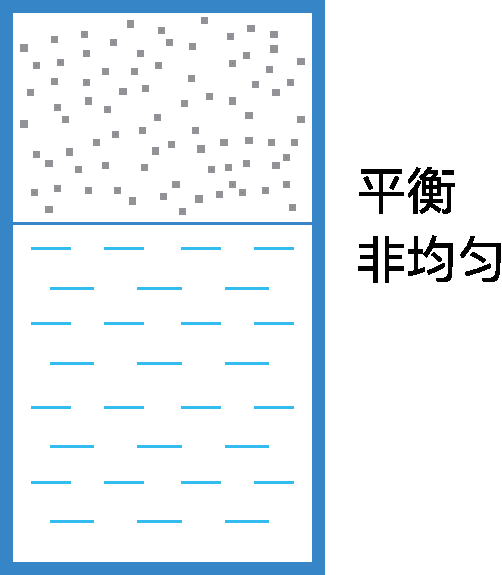
\includegraphics[width=0.4\linewidth]{pic/平衡与均匀.pdf}
	\captionof{figure}{平衡与均匀的区别}
	\label{ph1}
\end{minipage}%
\begin{minipage}[c]{0.5\linewidth}
	\centering
	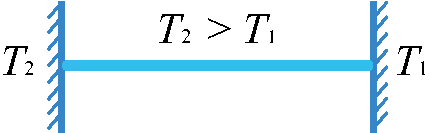
\includegraphics[width=0.7\linewidth]{pic/平衡与稳定.pdf}
	\captionof{figure}{平衡与稳定的区别}
	\label{ph2}
\end{minipage}%
}
}

\hspace*{1em} 平衡与稳定
\begin{myitemize}
	\item 平衡是无外界影响条件下状态不随时间改变\vspace*{-0.5em}
	\item 稳定只是状态不随时间改变
\end{myitemize}
]

\noindent 2. 平衡的条件
\begin{itemize}
	\item \dy[热平衡条件]{RPHTJ}:系统内部及系统与外界之间不存在温差。
	\item \dy[力平衡条件]{LPHTJ}:系统内部及系统与外界之间不存在力差。
	\item \dy[相平衡条件]{XPHTJ}:系统内部及系统与外界之间不存在化学势差。
	\item \dy[化学平衡条件]{HXPHTJ}:系统内部及系统与外界之间不存在化学势差。
\end{itemize}

\theorem[热力学平衡条件]
系统内部及系统与外界之间不存在温差、力差和化学势差。\index{RLXPHTJ@热力学平衡条件}\\

\noindent 7. 平衡的本质
\begin{itemize}
	\item 平衡的本质是\textbf{势平衡}。
	\item 势差会破坏平衡状态。
\end{itemize}

\section{状态参数}
\subsection{状态参数}
\noindent 1. 状态参数的概念

\defination[状态参数]
描述热力系统所处平衡状态的宏观物理量成为\dy[状态参数]{ZTCS}。\\

\noindent 2. 状态参数的属性
\begin{itemize}
	\item 状态参数具有\textbf{宏观性}。
	\item 某一状态具有\textbf{多个状态参数},如温度、压力、体积等。
	\item 某一状态参数在给定状态下具有\textbf{单值性}。具体而言:
	\begin{itemize}
		\item 在物理上表现为
		\begin{itemize}
			\item 状态一定则所有状态参数一定。
			\item 状态变化则至少一个状态参数变化。
			\item 状态参数的变化只取决于始末态而与路径无关。
		\end{itemize}
		\item 在数学上表现为
		\begin{itemize}
			\item 状态参数是点函数。
			\item 微分是全微分。
			\item 积分与路径无关。
		\end{itemize}
	\end{itemize}
\end{itemize}

\noindent 3. 状态参数的应用
\begin{itemize}
	\item 状态参数用来描述平衡状态下的系统
	\item 平衡状态下的均匀系统可用于一组统一的并具有确定数值的状态参数来描述。
	\item 平衡状态下的非均匀系统应先分为几个均匀部分再分别用一组统一的并具有确定数值的状态参数来分析。
\end{itemize}

\noindent 4. 状态参数的分类
\begin{itemize}
	\item \dy[广延参数]{GYCS}:与系统内所含物质的数量有关的量。例如:体积$V$、能量$E$等,这类参数具有\textbf{可加性}。
	\begin{itemize}
		\item \dy[比参数]{BCS}:单位质量的广延参数,具有强度参数的性质。例如比体积$v$、比能量$e$等。
		\begin{itemize}
			\item 对于均匀系统:比参数等于广延参数除以质量
			\item 对于非均匀系统:比参数等于广延参数对质量的微商。
		\end{itemize}
		\item \dy[摩尔参数]{MECS}:单位物质的量的广延参数,具有强度参数的性质。例如:摩尔体积$V_\text{m}$、摩尔能量$E_\text{m}$等。
		\begin{itemize}
			\item 对于均匀系统,摩尔参数等于广延参数除以物质的量
			\item 对于非均匀系统,摩尔参数等于广延参数对物质的量的微商
		\end{itemize}
	\end{itemize}
	\item \dy[强度参数]{QDCS}:与系统内所含物质的数量无关的量。例如:温度$T$、压力$p$等。这类参数具有\textbf{不可加性}。
\end{itemize}

\subsection{温度}
\noindent 1. 温度的概念

\defination[热平衡]
若冷热程度不同的物体接触,即发生热量传递,但足够长时间以后二者将达到相同的冷热程度,不再发生热量传递,处于\dy[热平衡]{RPH}。

\theorem[热力学第零定律]
与第三个系统处于热平衡的两个系统,彼此也处于热平衡。

\defination[温度]
描述一个系统和与之处于热平衡的其他系统之间的宏观特性的物理量称为\dy[温度]{WD}。温度可以用以确定一个系统是否与其他系统处于热平衡。\\

\noindent 2. 温度的属性
\begin{itemize}
	\item 温度是\textbf{状态参数}
	\item 温度是系统内部及系统之间的\textbf{热平衡判据}
\end{itemize}

\noindent 3. 温度的测量
\begin{itemize}
	\item \textbf{依据}:关于热平衡的系统具有相同的温度
	\item 测量温度的仪器为\textbf{温度计}
	\item 温度计读数与所采用测温物质的某种物理特性一一对应
\end{itemize}

\noindent 4. 温度的标量

\defination[温标]
温度的数值表示方法称为温度的标度,称为\dy[温标]{WB}。

\begin{itemize}
	\item 经验温标
	\begin{itemize}
		\item 华氏温标($\degree \text{F}$)
		\item 摄氏温标($\degree \text{C}$)
		\item 朗肯温标($\degree \text{R}$)
	\end{itemize}
	\item 热力学温标
	\begin{itemize}
		\item 热力学绝对温标(K)
		\item 热力学摄氏温标($\degree \text{C}$)
	\end{itemize}
\end{itemize}

各个温标之间的转换公式为
\begin{align}
	t\degree \text{C} = T \text{K} -273.15\\
	t\degree \text{C} =  \dfrac{5}{9}(t\degree \text{F} -32)\\
	T\degree \text{R} = t\degree \text{F} +459.69
\end{align}


\subsection{压力}
\noindent 1. 压力的概念

{\defination[压力]
单位面积上所受的法向力称为\dy[压力]{YL}。\\}

\noindent 2. 压力的测量
\begin{itemize}
	\item 仪器:压力计
	\item \dy[绝对压力$p$]{JDYL}:系统的真实压力。
	\item \dy[环境压力$p_\text{b}$]{HJYL}:外界的压力。
	\item \dy[表压力$p_\text{e}, p_\text{g}$]{BYL}:绝对压力高于环境压力时压力计的读数。
	\item \dy[真空度$p_\text{v}$]{ZKD}:绝对压力低于环境压力时压力计的读数。
	\item 计算公式
	\begin{equation}
		p=
		\begin{cases}
			p_\text{b} + p_\text{e} \quad (p>p_\text{b})\\
			p_\text{b} - p_\text{v} \quad (p<p_\text{b})\\
		\end{cases}
	\end{equation}
\end{itemize}

\noindent 3. 压力的单位

压力单位及换算如下表\ref{压力单位及换算表}.
\begin{table}[!htb]
	\centering
	\setlength{\tabcolsep}{10mm}{
	\begin{tabular}{cc}
		\toprule
		单位 & 换算成Pa\\
		\midrule
		1 bar & $1 \times 10^5$  Pa\\
		1 atm & $1.01325 \times 10^5$  Pa\\ 
		1 at & $9.80665 \times 10^4$  Pa\\
		1 mmHg & $133.322$  Pa\\
		1 mm$\text{H}_2$O & $9.80665$  Pa\\
		\bottomrule
	\end{tabular}
}
\caption{压力单位及换算表}
\label{压力单位及换算表}
\end{table}

\subsection{独立状态参数}
\tdefination[独立状态参数]
若描述以确定的平衡状态的状态参数的最小数目为$I$个,则这$I$个状态参数称为系统的\dy[独立状态参数]{DLZTCS}。

\begin{itemize}
	\item 系统与外界的作用途径
	\begin{itemize}
		\item 质量交换的自由度:$k$种可变物质
		\item 功量交换的自由度:$l$种可作功的力学参数
		\item 热量交换的自由度:1
	\end{itemize}
	\item 系统状态的总自由度:
	\begin{equation}
		I=k+l+1
	\end{equation}
\end{itemize}

\examples 计算如下系统的独立状态参数数目:
\begin{enumerate}[\hspace*{2em}(1)]
	\item 化学成分不改变的$k$元定质量简单可压缩系统;
	\item 具有$k$种可变物质的$k$元简单可压缩系统;
	\item 单元定质量简单可压缩系统;
	\item 单元变质量简单可压缩系统。
\end{enumerate}

\solve 
\begin{enumerate}[\hspace*{2em}(1)]
	\item $I=k+l+1=0+1+1=2.$
	\item $I=k+l+1=k+1+1=k+2.$
	\item $I=k+l+1=0+1+1=2.$
	\item $I=k+l+1=1+1+1=3.$
\end{enumerate}

\subsection{状态方程}
\tdefination[状态方程]
确定一个平衡状态有$I$个独立状态参数,平衡状态下其他状态参数一定是这$I$个独立状态参数的函数:
\begin{equation}
	X = X(x_1,x_2,\cdots,x_I)
\end{equation}
均匀系统处于平衡状态时,反映状态参数之间关系的方程称为\dy[状态方程]{ZTFC}
\begin{equation}
	F(x_1,x_2,\cdots,x_I,X)=0
\end{equation}
温度是基本状态参数,常在温度以外的状态参数中选取独立状态参数,而把温度作为“其他状态参数”,得到以下常见的状态方程:
\begin{equation}
	\varphi(x_1,x_2,\cdots,x_I,T) = 0
\end{equation}

\noindent 例如:
\begin{itemize}
	\item 对于具有$k$种可变物质的$k$元简单可压缩系统,$I=k+1+1=k+2$,其状态方程为
	\begin{equation}
		\varphi_1 (m_1,m_2,\cdots,m_k,p,V,T) = 0
	\end{equation}
	\item 对于单元变质量简单可压缩系统,$I=1+1+1=3$,其状态方程为
	\begin{equation}
		\varphi_2(m,p,V,T) = 0
	\end{equation}
	这与理想气体状态方程
	\begin{equation}
		pV=mRT
	\end{equation}
相吻合。
\end{itemize}

\subsection{状态图}
\noindent 1. 状态图的定义

\defination[状态图]
热力系统处于平衡状态时,独立状态参数作为坐标组成的坐标图称为\dy[状态图]{ZTT}。

\section{热力过程}

\subsection{过程}
\noindent 1. 过程的定义

\defination[过程]
热力状态的连续变化称为\dy[热力过程]{RLGC},简称\dy[过程]{GC}。\vspace*{0.5em}

\noindent 2. 过程的本质

过程的本质是平衡状态被势差破坏后经历的\textbf{一系列非平衡状态}。\vspace*{0.5em}

\noindent 3. 研究方法

对实际过程进行简化,建立理想模型,进而用状态参数描述实际过程。\\

\subsection{准平衡过程}

\tdefination[准平衡状态]
无限接近于平衡状态的统一状态参数来描述的状态称为\dy[准平衡状态]{ZPHZT}。

\defination[准平衡过程]
从某一初始平衡状态经历一系列准平衡状态连续地变化到另一个最终平衡状态的过程\dy[准平衡过程]{ZPHGC}。
\vspace*{1em}

\subsection{过程图}
\tdefination[过程图]
热力系统经历准平衡过程时,以曲线表示过程的状态图称为\dy[过程图]{GCT}。
\vspace*{1em}

\section{热力循环}
\subsection{循环}
\tdefination[循环]
热力系统从初始状态出发经历一系列过程之后又回复到初始状态,这一系列过程的综合称为\dy[热力循环]{RLXH},简称\dy[循环]{XH}。\vspace*{0.5em}

\noindent 分类\vspace*{-1em}
\begin{itemize}
	\item 经历一个循环系统对外界作出功量的循环称为\dy[正向循环]{ZXXH},也称为\dy[动力循环]{DLXH}。
	\item 经历一个循环外界对系统作出功量以实现把热量从低温热源传递到高温热源的循环称为\dy[逆向循环]{NXXH},也称为\dy[制冷循环]{ZLXH}或\dy[供热循环]{GRXH}。
\end{itemize}


\noindent 意义

热力系统经过循环回复到初始状态,就能按相同过程不断重复,因而能连续不断地作功,或连续不断地制冷或供热。
\vspace*{1em}

\subsection{循环图}

\tdefination[循环图]
以封闭曲线表示循环的状态图称为\dy[循环图]{XHT}。

\newpage
\begin{figure}[!htb]
		\centering
		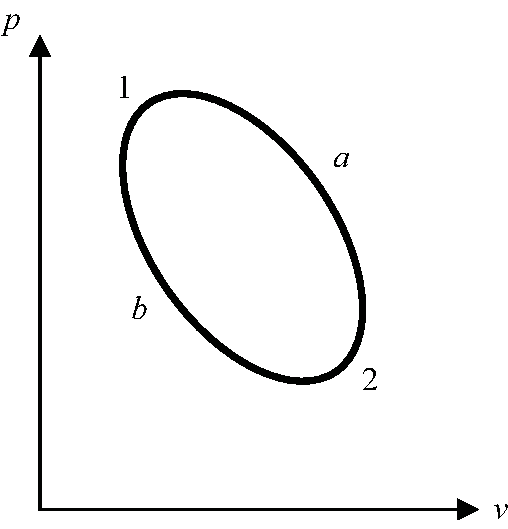
\includegraphics[width=0.4\linewidth]{pic/数学描述曲线.pdf}
		\caption{循环图}
		\label{循环图}
\end{figure}

\noindent 特点\vspace*{-1em}
\begin{itemize}
	\item 正向循环的循环图为顺时针方向
	\item 逆向循环的循环图为逆时针方向
\end{itemize}
